
%(BEGIN_QUESTION)
% Copyright 2010, Tony R. Kuphaldt, released under the Creative Commons Attribution License (v 1.0)
% This means you may do almost anything with this work of mine, so long as you give me proper credit

Sketch connecting wires to show how to simulate a {\it thermocouple} signal to the input of this electronic temperature transmitter using a potentiometer and a battery:

$$\includegraphics[width=15.5cm]{i00591x01.eps}$$

Assume the transmitter is properly configured for thermocouple input, and that the potentiometer is of sufficient precision and resolution that there is no need to connect it to any other resistors to form a network.

\underbar{file i00591}
%(END_QUESTION)





%(BEGIN_ANSWER)

$$\includegraphics[width=15.5cm]{i00591x02.eps}$$

Any correct solution will include these attributes:

\begin{itemize}
\item{} 1.5 volt battery connected across whole span of potentiometer
\item{} Wiper terminal connected to one input terminal of transmitter
\item{} Other transmitter input terminal connected to proper pole of battery (polarity needs to match)
\end{itemize}

%(END_ANSWER)





%(BEGIN_NOTES)

{\bf This question is intended for exams only and not worksheets!}.

%(END_NOTES)


